\chapter{Experiments}
\label{c:experiments}
\IMRADlabel{results}



In this chapter we will present all environments we experimented with as well as \emph{Hyper-Experiments}, \ac{ie} experiments with the hyperparameters and their influence on the algorithm performance (in terms of the prediction error and similar metrics, not the computing time).

\section{Environments and Experiment Setup}
	We will not introduce to you the environments and the setup for each environment that we used. We will not discuss any results here,see~\autoref{c:discussion} for that. Do generate the data, you have to run the file \texttt{src/data.py} with the desired experiment ID as the first argument, \ac{eg} \texttt{python src/data.py pendulum\_damped}. If no argument is given, a regeneration of the data from all experiments is triggered. For each of the following environments we summarize the most important data about the environment at the start of the subsection, including the experiment ID.

	\subsection{Proof of Concept: Classic LGDS}
		\begin{itemize}
			\item Experiment ID: \texttt{lgds}
		\end{itemize}

		As a proof of concept and to empirically verify our proof on the exactness of the cubature rule and hence the similar expected performance for plain linear systems, we benchmark our algorithm against a simple linear system. The linear system has a two-dimensional state \( \vec{y} \coloneqq \begin{bmatrix} x_1 & x_2 \end{bmatrix}^T \) with the dynamics
		\begin{align*}
			\dot{x}_1 &= x_2 \\
			\dot{x}_2 &= -x_1
		\end{align*}
		The initial state \( \vec{s}_1 \) is sampled from a Gaussian with mean \( \begin{bmatrix} 0.1 & 0.2 \end{bmatrix}^T \) and covariance \( \diag\big(10^{-5}, 10^{-5}\big) \). The system is integrated using the implicit Runge-Kutta Radau~IIA~\cite{guglielmiImplementingRadauIIA2001} method with an evaluation interval of \( h = 0.1 \) for \( T = 240 \) time steps where only the first \( T_\train = 120 \) steps are used for training and the remaining \(120\) are used for validation. The raw data is shown in~\autoref{fig:envLgds}.

		As the system's eigenvalues \( -i \), \( i \) are purely imaginary, the integrated system rings around the equilibrium \( \begin{bmatrix} 0 & 0 \end{bmatrix}^T \) infinitely.

		\begin{figure}
			\centering
			\begin{subfigure}{0.5\linewidth}
				\centering
				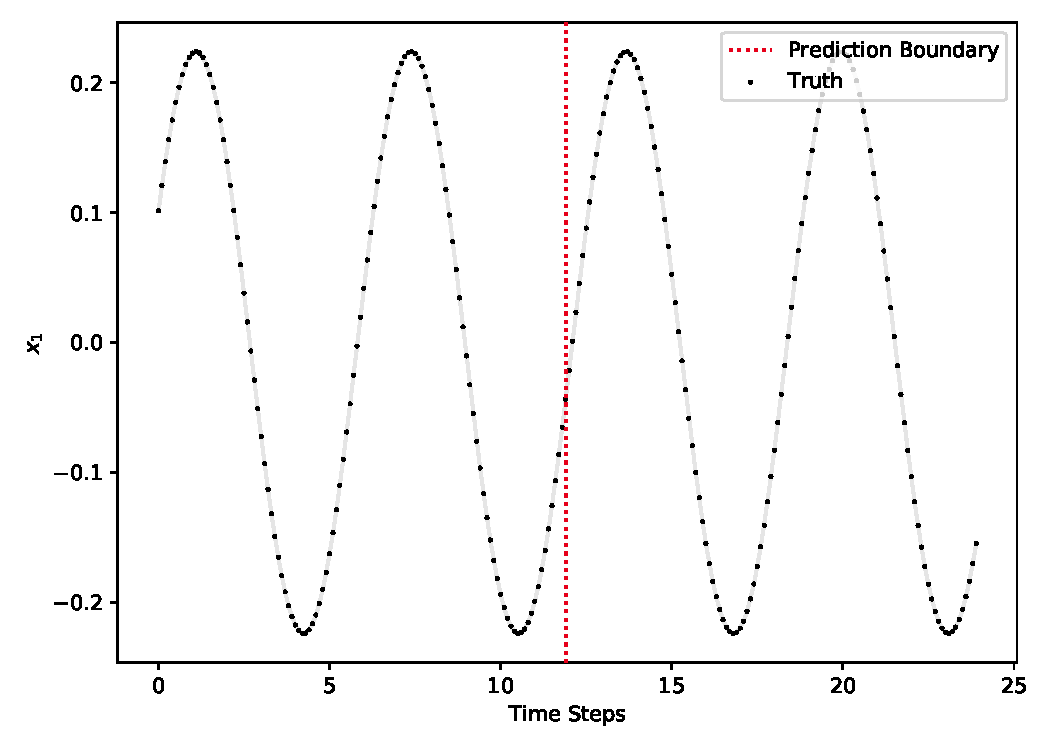
\includegraphics[width=\linewidth]{figures/experiments/environments/observations-lgds-N0-D0.pdf}
			\end{subfigure}%
			~
			\begin{subfigure}{0.5\linewidth}
				\centering
				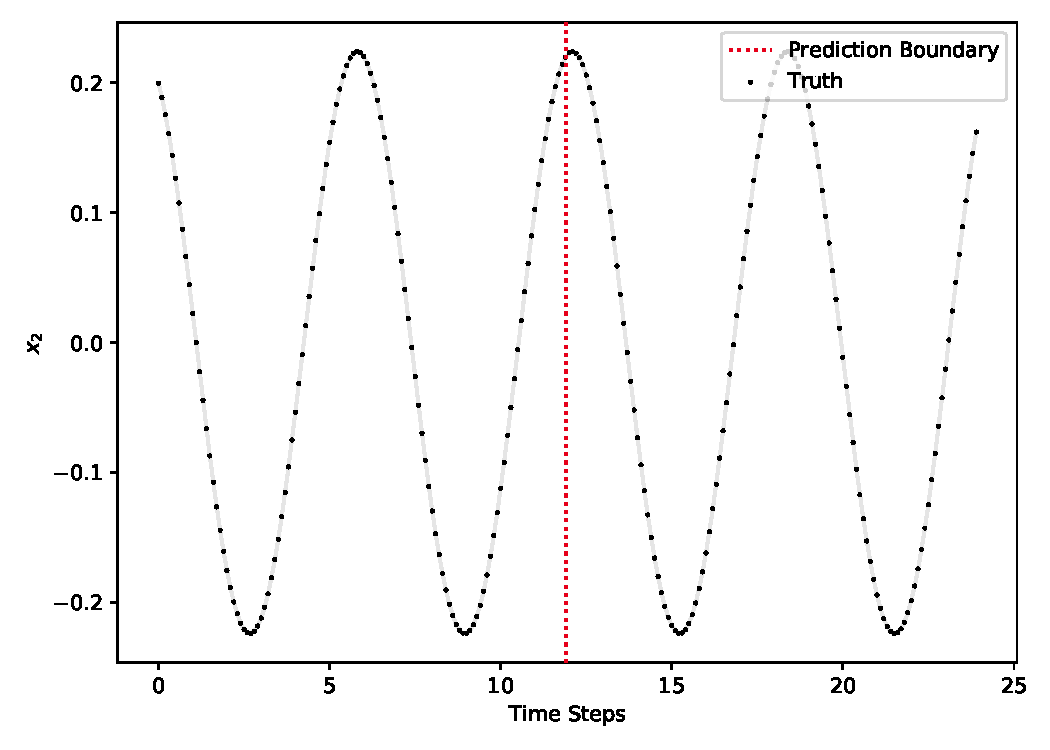
\includegraphics[width=\linewidth]{figures/experiments/environments/observations-lgds-N0-D1.pdf}
			\end{subfigure}
			\caption{Plot of the raw data used for training the proof-of-concept \ac{lgds} environment. The black dots represent the actual data points, all before the red prediction boundary are used for training, the rest for validation. The faint gray line emphasizes the connection between the data points and that they are actually generated from a dynamical system.}
			\label{fig:envLgds}
		\end{figure}
	% end

	\subsection{(Damped) Pendulum}
		\begin{itemize}
			\item Experiment ID: \texttt{pendulum} and \texttt{pendulum\_damped}
		\end{itemize}

		The first nonlinear system we look at is the (inverted) pendulum in both an undamped and a damped setting. For this experiment, we use the angular state \( \vec{y} = \begin{bmatrix} \theta & \dot{\theta} \end{bmatrix} \) where \(\theta\) is the displacement angle (see~\autoref{fig:envPendulumSketch}). The dynamics are specified by the \ac{ode}
		\begin{equation*}
			\ddot{\theta} = \sin\theta - d \dot{\theta}
		\end{equation*}
		that is solved using the Radau~IIA~\cite{guglielmiImplementingRadauIIA2001} \ac{ivp} integrator (after transforming the \ac{ode} in a first-order \ac{ode} system). The initial velocity is set to \(0\) and the initial position is sampled from a Gaussian with mean \( \pi/36 \) and variance \( \pi/8 \). This puts the pendulum in motion as it falls down from its initial position. For the undamped pendulum, we set \( d = 0 \). For both environments, we use an evaluation interval of \( h = 0.1 \) for \( T = 1000 \) time steps where only the first \( T_\train = 500 \) steps are used for training and the remaining \(500\) are used for validation. The raw data is shown in~\autoref{fig:envPendulum} for the undamped and~\autoref{fig:envPendulumDamped} for the damped pendulum.

		The damped pendulum is especially interesting as the system looses energy (\ac{ie} the sum of the kinetic and potential energy decreases over time) and Koopman theory in general has problems with finding embeddings that are able to encode energy loss\todo{citation needed}.

		\begin{figure}
			\centering
			\begin{subfigure}{0.5\linewidth}
				\centering
				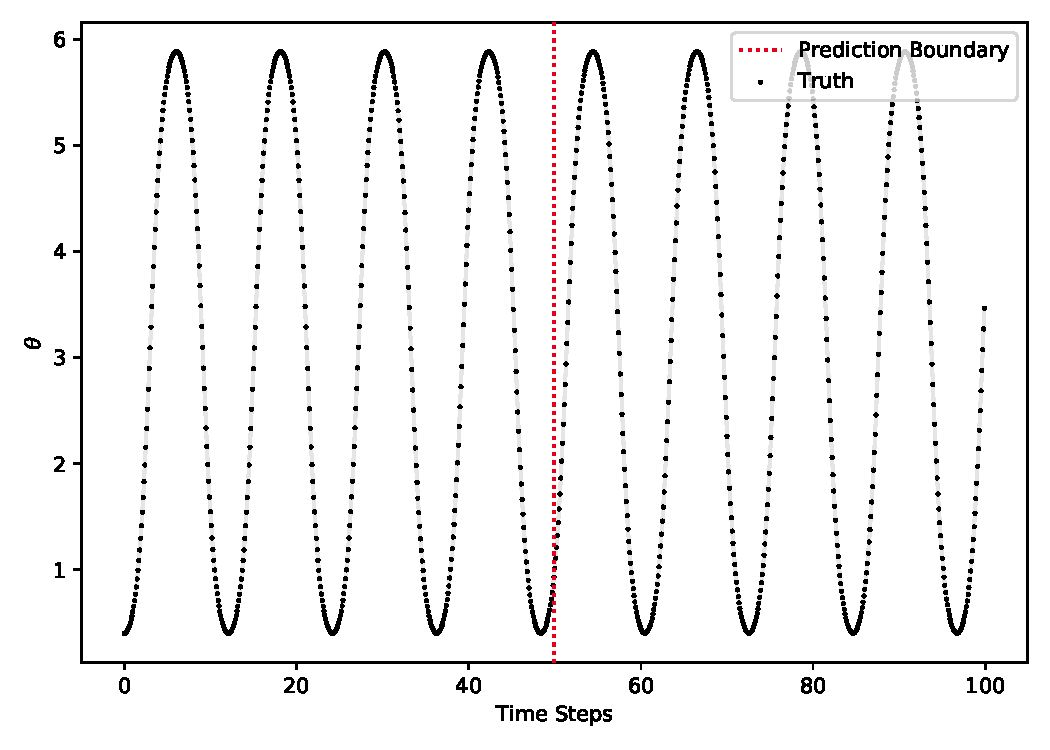
\includegraphics[width=\linewidth]{figures/experiments/environments/observations-pendulum-N0-D0.pdf}
			\end{subfigure}%
			~
			\begin{subfigure}{0.5\linewidth}
				\centering
				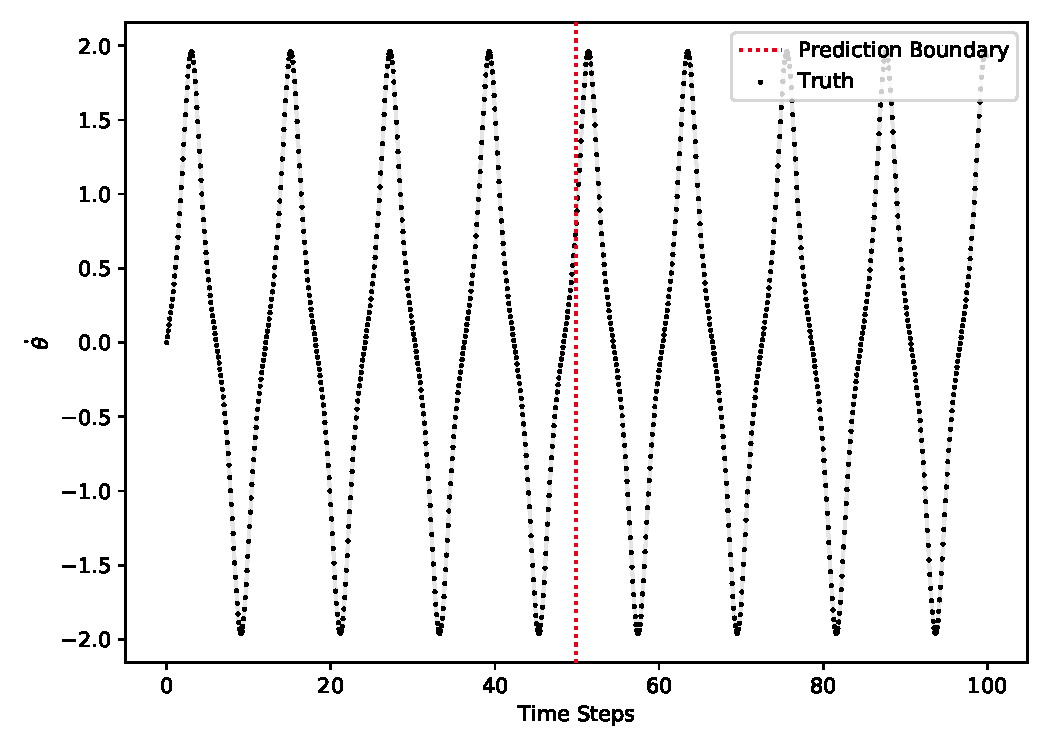
\includegraphics[width=\linewidth]{figures/experiments/environments/observations-pendulum-N0-D1.pdf}
			\end{subfigure}
			\caption{Plot of the raw data used for training the undamped pendulum environment. The black dots represent the actual data points, all before the red prediction boundary are used for training, the rest for validation. The faint gray line emphasizes the connection between the data points and that they are actually generated from a dynamical system.}
			\label{fig:envPendulum}
		\end{figure}
		\begin{figure}
			\centering
			\begin{subfigure}{0.5\linewidth}
				\centering
				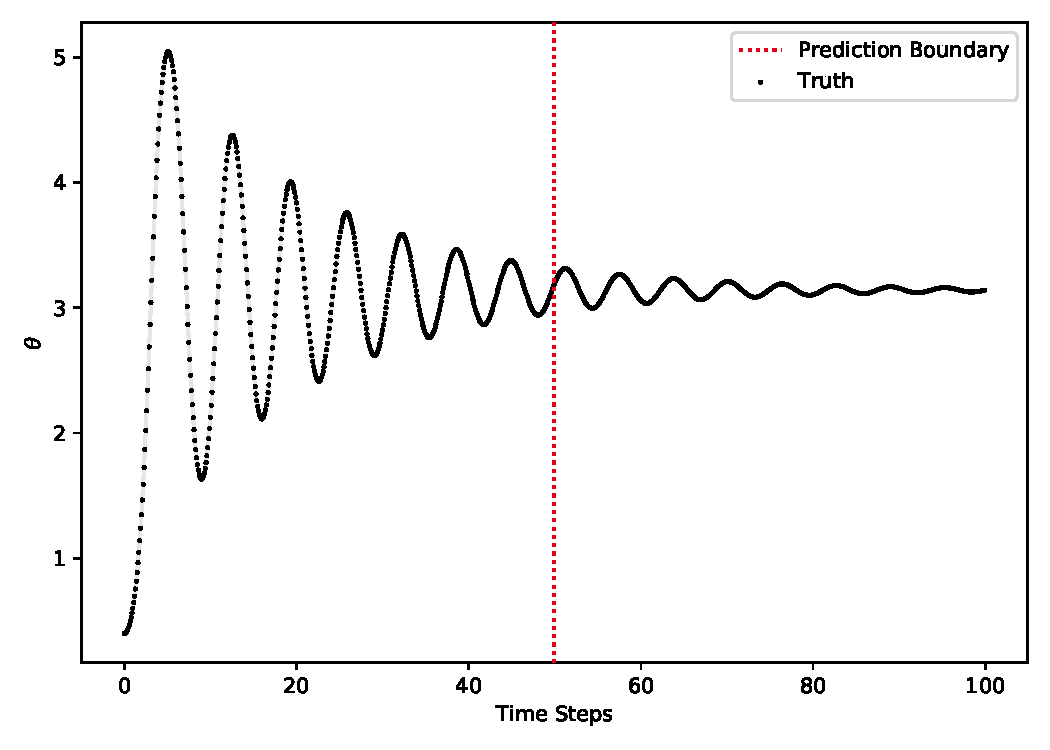
\includegraphics[width=\linewidth]{figures/experiments/environments/observations-pendulum-damped-N0-D0.pdf}
			\end{subfigure}%
			~
			\begin{subfigure}{0.5\linewidth}
				\centering
				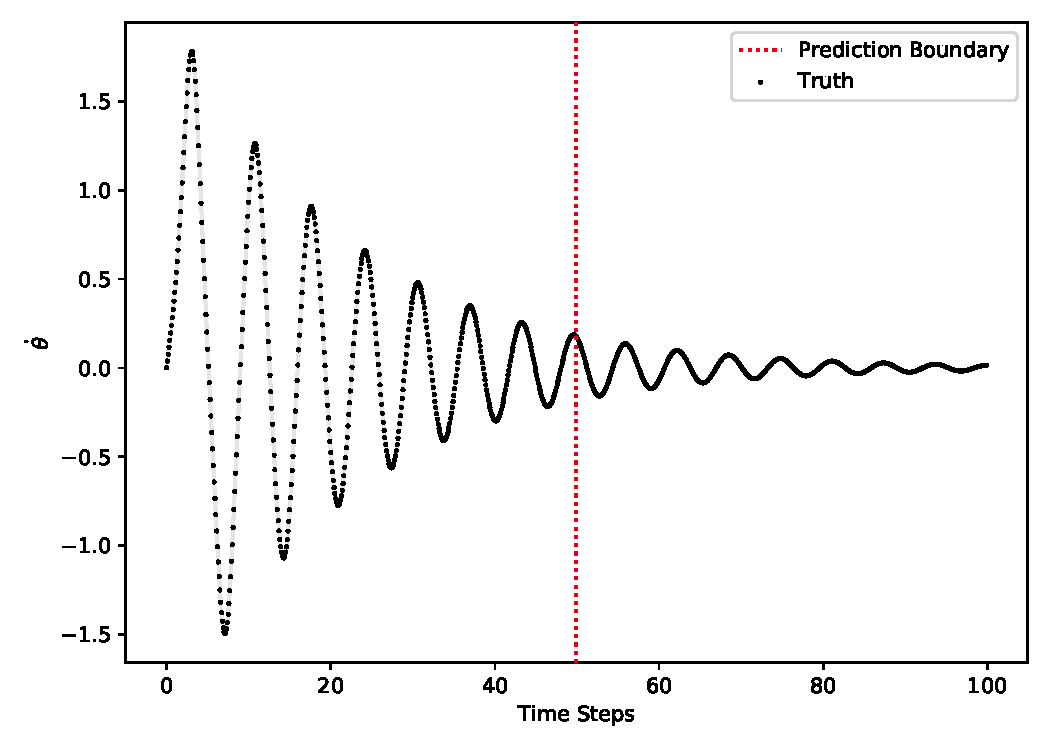
\includegraphics[width=\linewidth]{figures/experiments/environments/observations-pendulum-damped-N0-D1.pdf}
			\end{subfigure}
			\caption{Plot of the raw data used for training the damped pendulum environment. The black dots represent the actual data points, all before the red prediction boundary are used for training, the rest for validation. The faint gray line emphasizes the connection between the data points and that they are actually generated from a dynamical system.}
			\label{fig:envPendulumDamped}
		\end{figure}
	% end

	\subsection{Gym Pendulum}
		\begin{itemize}
			\item Experiment ID: \texttt{pendulum\_gym}
		\end{itemize}

		This is a sine/cosine version of the pendulum introduced before, but without damping. We use the environment of OpenAI Gym~\cite{brockmanOpenAIGym2016} for generating the data used for training. The motion equations are still the same as for the non-Gym pendulum
		\begin{equation*}
			\ddot{\theta} = \sin\theta
		\end{equation*}
		with \( d = 0 \) as the Gym pendulum does not include damping, but the state is defined as the sine and cosine of the angle:
		\begin{equation*}
			\vec{y} \coloneqq
				\begin{bmatrix}
					\cos\theta \\
					\sin\theta \\
					\dot{\theta}
				\end{bmatrix}
		\end{equation*}
		The Gym environment uses the Euler method for integrating the \ac{ode} with a step size of \( h = 0.05 \). We generate \( T = 100 \) time steps of which \( T_\train = 50 \) are used for training and the other \(50\) for validation. The raw data is shown in~\autoref{fig:envPendulumGym}.

		\begin{figure}
			\centering
			\begin{subfigure}{0.5\linewidth}
				\centering
				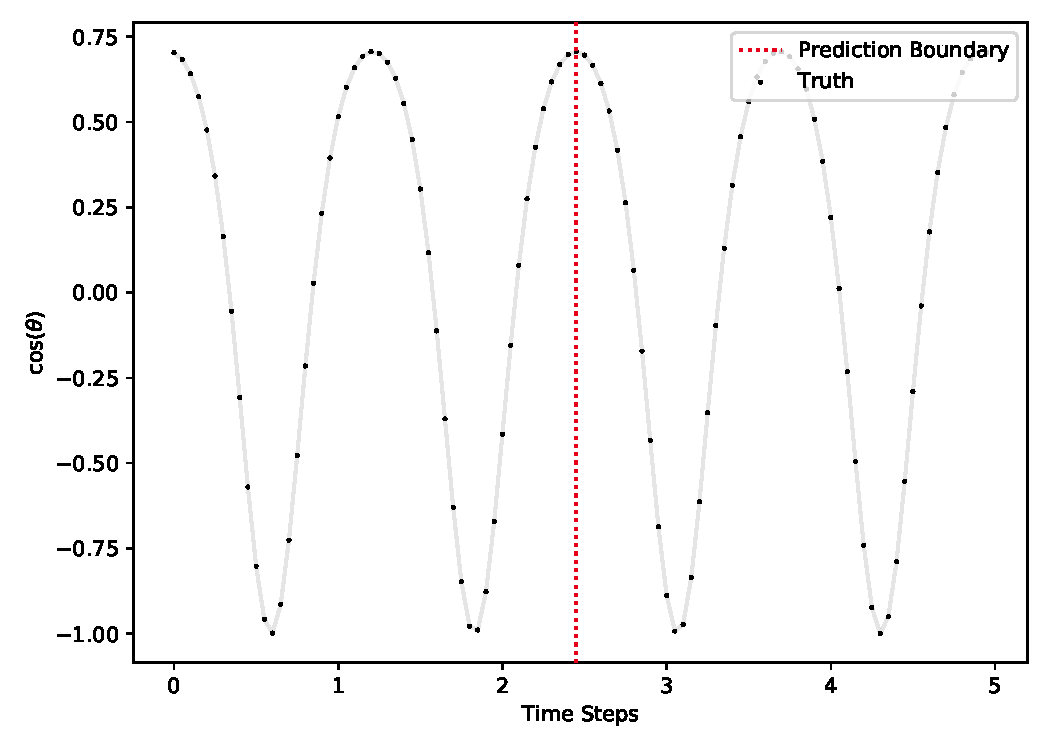
\includegraphics[width=\linewidth]{figures/experiments/environments/observations-pendulum-gym-N0-D0.pdf}
			\end{subfigure}%
			~
			\begin{subfigure}{0.5\linewidth}
				\centering
				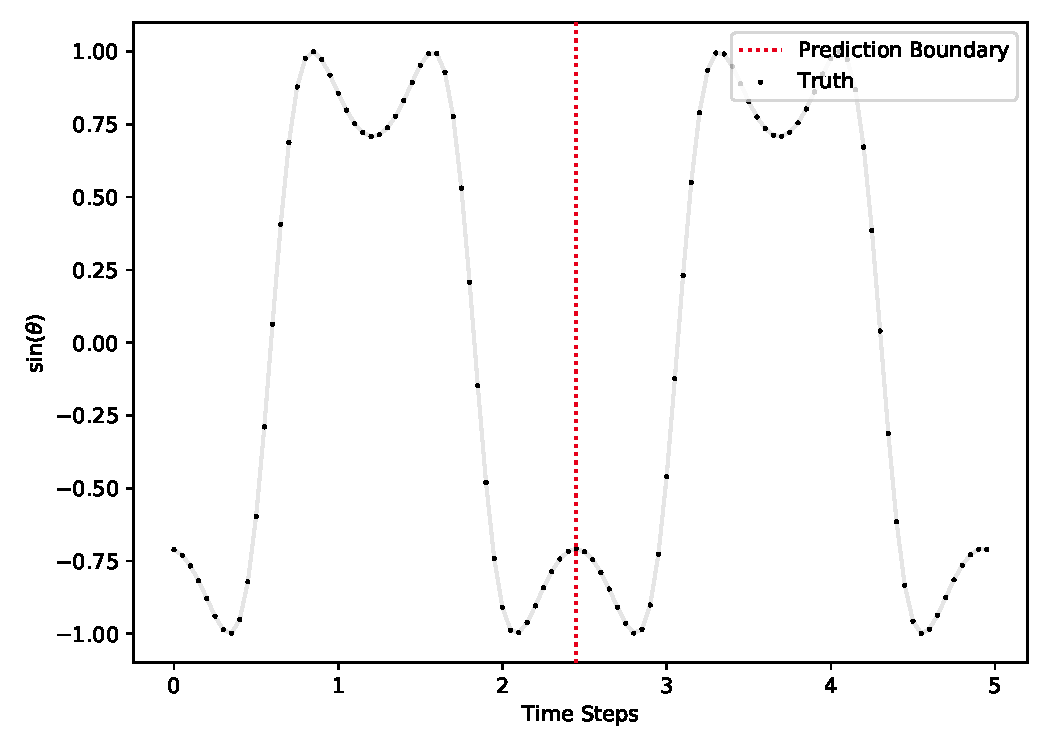
\includegraphics[width=\linewidth]{figures/experiments/environments/observations-pendulum-gym-N0-D1.pdf}
			\end{subfigure} \\
			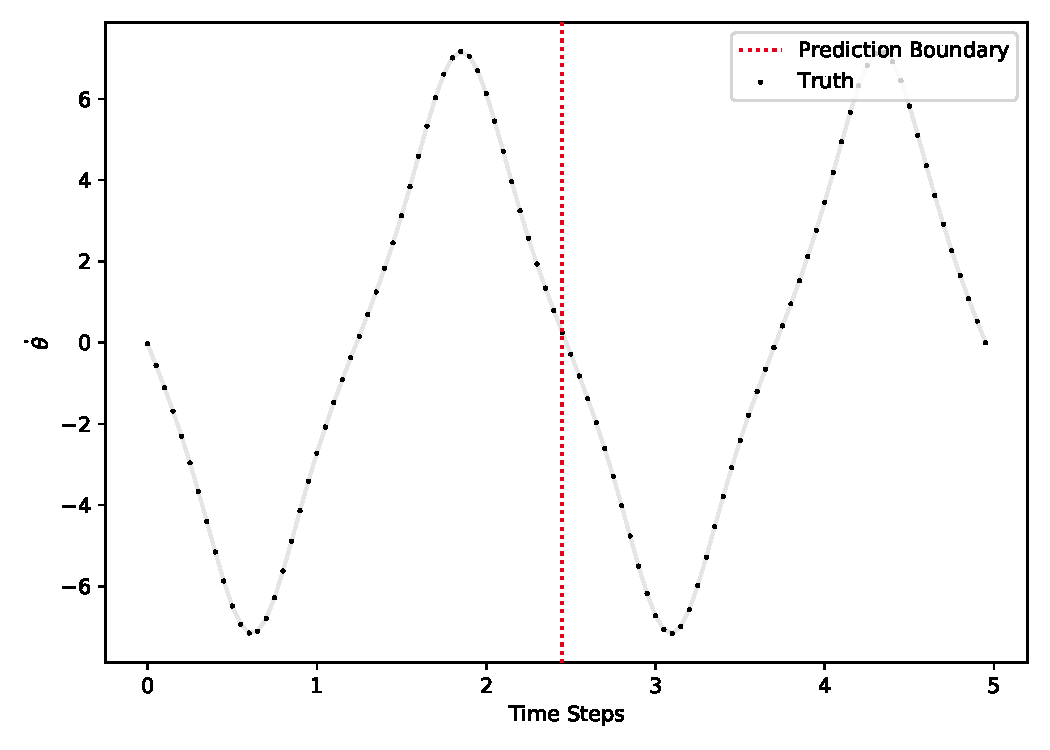
\includegraphics[width=0.5\linewidth]{figures/experiments/environments/observations-pendulum-gym-N0-D2.pdf}
			\caption{Plot of the raw data used for training the Gym pendulum environment. The black dots represent the actual data points, all before the red prediction boundary are used for training, the rest for validation. The faint gray line emphasizes the connection between the data points and that they are actually generated from a dynamical system.}
			\label{fig:envPendulumGym}
		\end{figure}
	% end

	\subsection{Gym Cartpole}
		\begin{itemize}
			\item Experiment ID: \texttt{cartpole\_gym}
		\end{itemize}

		The second last environment we run experiment on is the cartpole environment. In the cartpole environment, an inverted pendulum is build on a (typically controlled, but otherwise freely movable) cart. If the pendulum falls town, the torque on the joint is translated into a force moving the cart around. This creates nonlinear coupling and therefore highly nonlinear dynamics. A sketch of the cartpole environment is given in~\autoref{fig:envCartpoleGymSketch}. As for the previous pendulum, we rely on the cartpole implementation of Gym. We slightly modified the environment to be uncontrolled, as the environment usually has discrete actions for pushing the cart left or right. This modification is shown in~\autoref{lst:uncontrolledCartPole}. The state of the environment is given as
		\begin{equation*}
			\vec{y} \coloneqq
				\begin{bmatrix}
					x \\
					\dot{x} \\
					\theta \\
					\dot{\theta}
				\end{bmatrix}
		\end{equation*}
		where \(x\) is the cart position, \(\dot{x}\) is the cart velocity, \(\theta\) is the pole angle and \(\dot{\theta}\) is the angular velocity. The implemented equations of movement, taken from~\cite{florianCorrectEquationsDynamics2005}, are given as
		\begin{align*}
			\ddot{\theta} &= \frac{g \sin\theta + \cos\theta \Big(\! \frac{-F - m_p \ell \dot{\theta}^2 \sin\theta}{m_c + m_p} \!\Big)}{\ell \Big(\! \frac{4}{3} - \frac{m_p \cos^2\theta}{m_c + m_p} \!\Big)} \\
			\ddot{x} &= \frac{F + m_p \ell \big( \dot{\theta}^2 \sin\theta - \ddot{\theta} \cos\theta \big)}{m_c + m_p}
		\end{align*}
		where \( g = \SI{9.81}{\meter\per\second\squared} \) is the gravitational acceleration, \( m_p = \SI{0.1}{\kilogram} \) and \( m_c = \SI{1}{\kilogram} \) are the masses of the pole and cart, respectively, \( 2\ell = \SI{1}{\meter} \) is the pole length and \( [F] = \si{\newton} \) is the external (control) force acting on the cart that we set to \( \SI{0}{\newton} \). The Gym environment uses the Euler method for integrating the \ac{ode} with a step size of \( h = 0.02 \). We generate \( T = 300 \) time steps of which we use \( T_\train = 150 \) for training and the remaining \(150\) steps for validation. The raw data is shown in~\autoref{fig:envCartpoleGym}.

		\begin{lstlisting}[caption={Modification of Gym's cartpole environment to get an uncontrolled cartpole.}, label=lst:uncontrolledCartPole]
from gym.envs.classic_control import CartPoleEnv

class UncontrolledCartPole(CartPoleEnv):
	def __init__(self):
	super().__init__()

	self.force_mag = 0.0
		\end{lstlisting}

		\begin{figure}
			\centering
			\tikzCartpole
			\caption{Illustration of the cartpole environment. The cart has mass \(m_c\), the pole \(m_p\) with length \(L\). The cart can move freely on the \(x\) axis, while the pendulum can swing freely around the center of the cart, causing it to move.}
			\label{fig:envCartpoleGymSketch}
		\end{figure}

		\begin{figure}
			\centering
			\begin{subfigure}{0.5\linewidth}
				\centering
				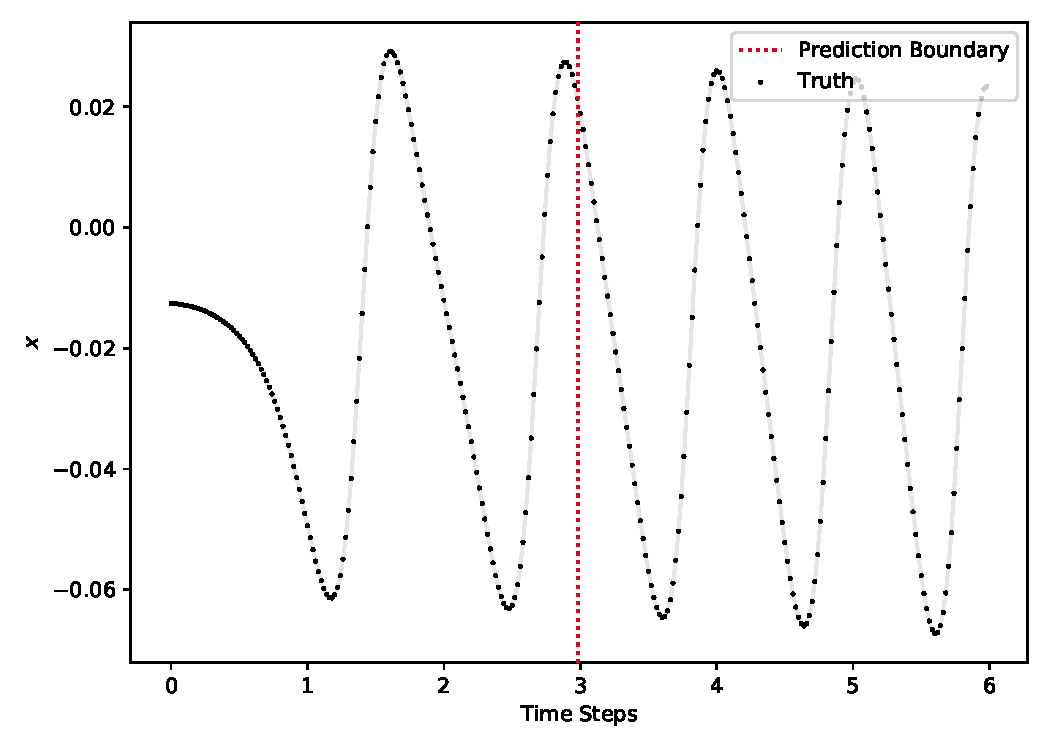
\includegraphics[width=\linewidth]{figures/experiments/environments/observations-cartpole-gym-N0-D0.pdf}
			\end{subfigure}%
			~
			\begin{subfigure}{0.5\linewidth}
				\centering
				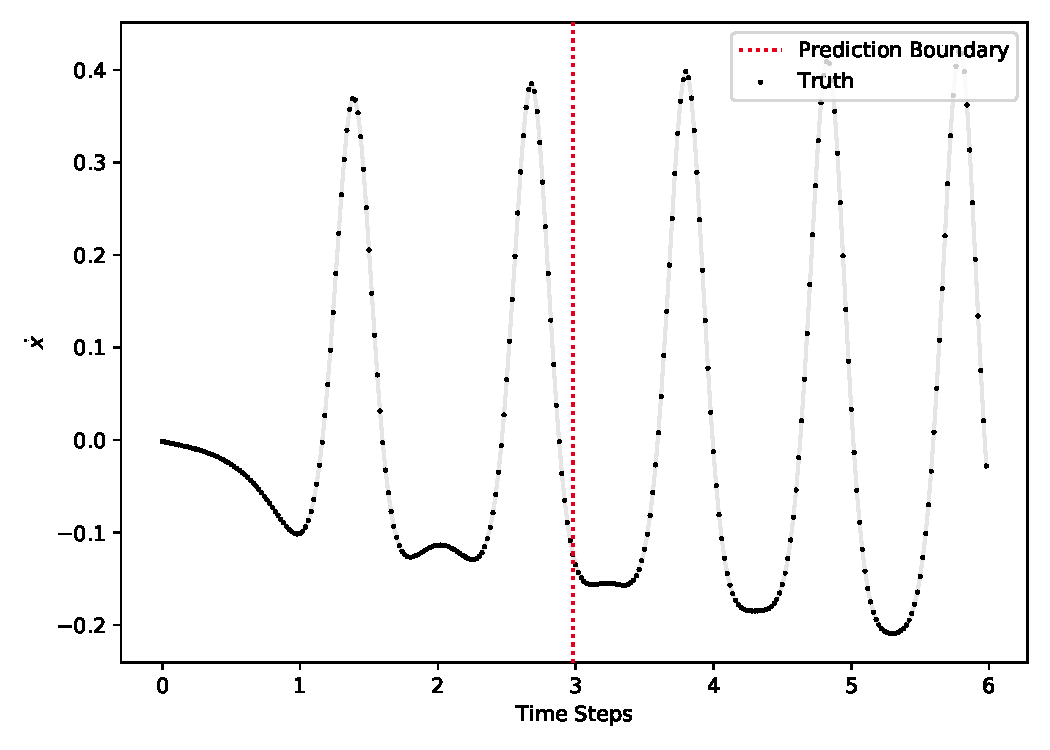
\includegraphics[width=\linewidth]{figures/experiments/environments/observations-cartpole-gym-N0-D1.pdf}
			\end{subfigure} \\
			\begin{subfigure}{0.5\linewidth}
				\centering
				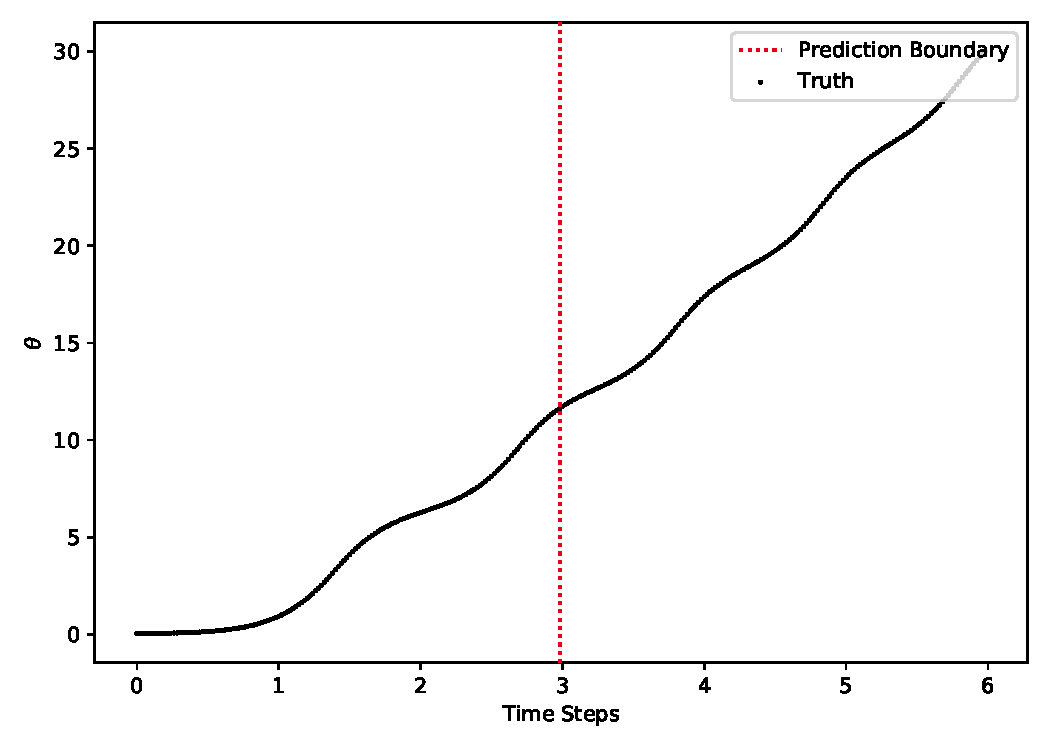
\includegraphics[width=\linewidth]{figures/experiments/environments/observations-cartpole-gym-N0-D2.pdf}
			\end{subfigure}%
			~
			\begin{subfigure}{0.5\linewidth}
				\centering
				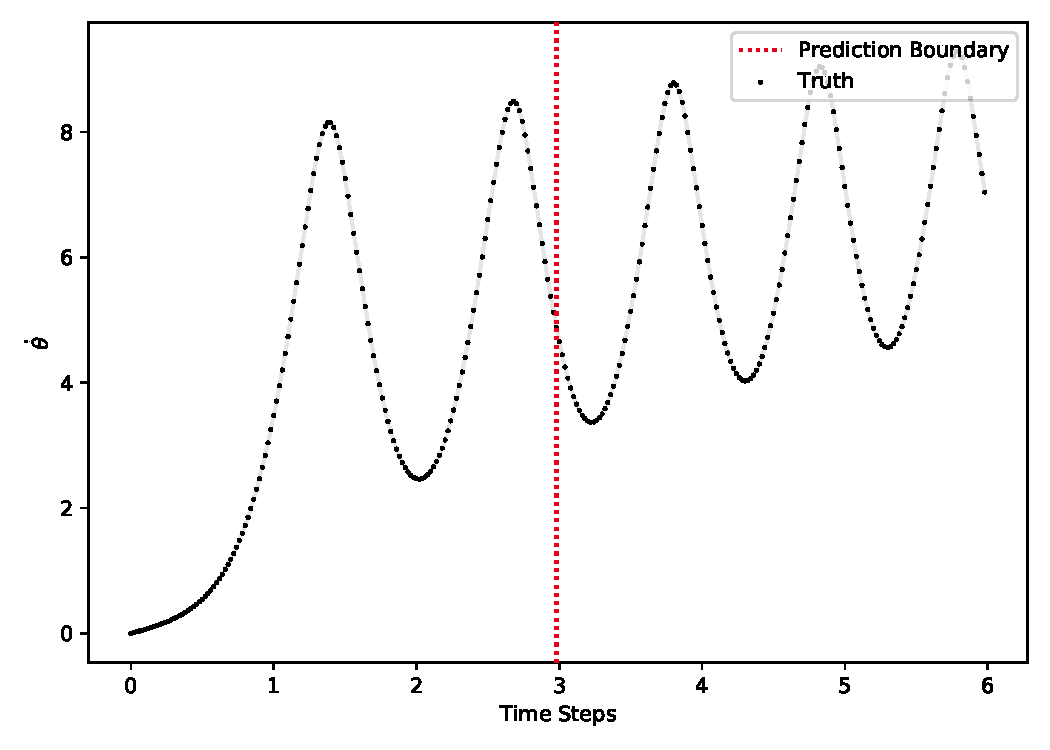
\includegraphics[width=\linewidth]{figures/experiments/environments/observations-cartpole-gym-N0-D3.pdf}
			\end{subfigure}
			\caption{Plot of the raw data used for training the Gym cartpole environment. The black dots represent the actual data points, all before the red prediction boundary are used for training, the rest for validation. The faint gray line emphasizes the connection between the data points and that they are actually generated from a dynamical system.}
			\label{fig:envCartpoleGym}
		\end{figure}
	% end

	\subsection{Gym Double Pendulum}
		\begin{itemize}
			\item Experiment ID: \texttt{acrobot\_gym}
		\end{itemize}

		The last environment we test is the double pendulum, implemented in Gym as the \emph{acrobot} (as for the cartpole, we removed all control inputs and modified the initial state to start on top rather than hanging straight down, see~\autoref{lst:topAcrobot}). The double pendulum consists of a pendulum on a fixed joint and a second pendulum attached to the end of the first pendulum. This creates highly nonlinear coupling and is the most common example of a chaotic system~\cite{shinbrotChaosDoublePendulum1992}. We observe the state vector
		\begin{equation*}
			\vec{y} \coloneqq
				\begin{bmatrix}
					\cos\varphi_1 \\
					\sin\varphi_1 \\
					\cos\varphi_2 \\
					\sin\varphi_2 \\
					\dot{\varphi}_1 \\
					\dot{\varphi}_2
				\end{bmatrix}
		\end{equation*}
		where \(\varphi_1\) and \(\varphi_2\) are the displacement of the first and second joint, respectively. See~\autoref{fig:envDoublePendulumGymSketch}) for a sketch of the double pendulum. The governing equations of motion are given as:´
		\begin{align*}
			\ddot{\varphi}_1 &= \frac{g (\sin\varphi_2 \, \cos\varphi_\Delta - \mu \sin\varphi_1) - (\ell_2 \dot{\varphi}_2^2 + \ell_1 \dot{\varphi}_1^2 \cos\varphi_\Delta) \sin\varphi_\Delta}{\ell_1 (\mu - \cos^2\varphi_\Delta)} \\
			\ddot{\varphi}_2 &= \frac{g \mu (\sin\varphi_2 \, \cos\varphi_\Delta - \mu \sin\varphi_1) + (\mu \ell_1 \dot{\varphi}_1^2 + \ell_2 \dot{\varphi}_2^2 \cos\varphi_\Delta) \sin\varphi_\Delta}{\ell_2 (\mu - \cos^2\varphi_\Delta)}
		\end{align*}
		with \( \varphi_\Delta \coloneqq \varphi_1 - \varphi \), \( \mu \coloneqq 1 + m_1/m_2 \) where \( g = \SI{9.8}{\meter\per\second\squared} \) is the gravitational acceleration, \( m_1 = \SI{1}{\kilogram} \) and \( m_2 = \SI{1}{\kilogram} \) are the masses of the two links and \( \ell_1 = \SI{1}{\meter} \) and \( \ell_2 = \SI{1}{\meter} \) are the lengths of the two links. The Gym environment uses a \ac{rk4} for integrating the \ac{ode} with an evaluation interval of \( h = 0.2 \). We modified the initial position to be drawn from a Gaussian with mean \( \pi \) and standard deviation \( \pi/8 \) and the initial velocity to be drawn from a uniform distribution in the interval \( [-0.1, 0.1] \). We generate \( T = 100 \) time steps of which we use \( T_\train = 75 \) for training and the remaining \(25\) for validation. The raw data is shown in~\autoref{fig:envDoublePendulumGym}.

		\begin{lstlisting}[caption={Modification of Gym's acrobot environment to start at the top instead of hanging down.}, label=lst:topAcrobot]
import numpy as np
from gym.envs.classic_control import AcrobotEnv

class ModifiedAcrobotEnv(AcrobotEnv):
	def __init__(self):
		super().__init__()

	def reset(self):
		position = self.np_random.normal(np.pi, np.pi / 8.0, size=(2,))
		velocity = self.np_random.uniform(low=-0.1, high=0.1, size=(2,))
		self.state = np.concatenate([position, velocity], axis=0)
		return self._get_ob()
		\end{lstlisting}

		\begin{figure}
			\centering
			\tikzDoublePendulum
			\caption{Illustration of the double pendulum environment. The pendulums have lengths \(\ell_1\) and \(\ell_2\) with the masses \(m_1\) and \(m_2\) attached to the respective ends. The inner pendulum can swing freely around the center while the other pendulum can swing freely around the end of the inner pendulum. Hence fixing one of the pendulums would transform the system back to a simple pendulum. If both pendulums can swing, the system is chaotic.}
			\label{fig:envDoublePendulumGymSketch}
		\end{figure}

		\begin{figure}
			\centering
			\begin{subfigure}{0.5\linewidth}
				\centering
				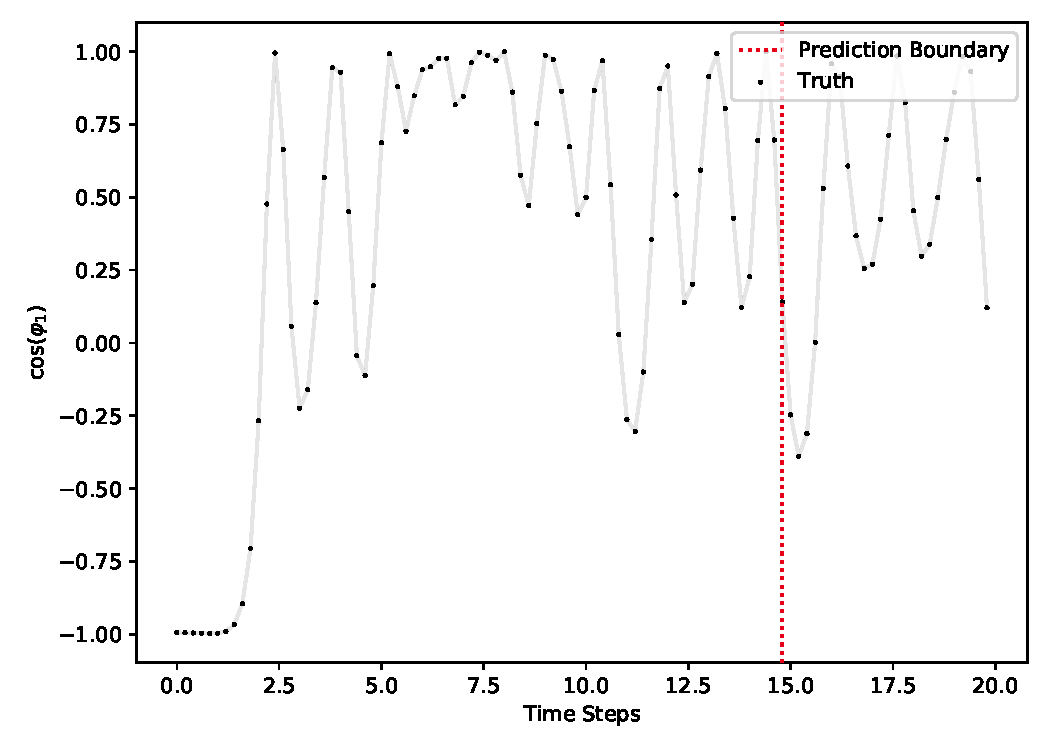
\includegraphics[width=\linewidth]{figures/experiments/environments/observations-acrobot-gym-N0-D0.pdf}
			\end{subfigure}%
			~
			\begin{subfigure}{0.5\linewidth}
				\centering
				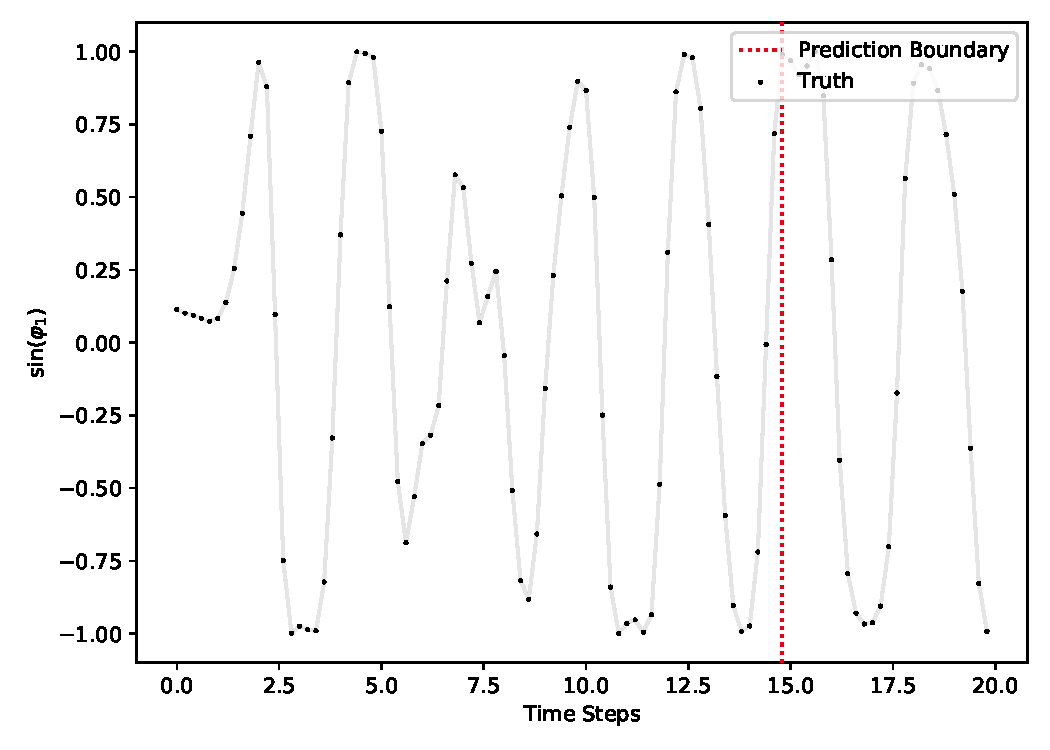
\includegraphics[width=\linewidth]{figures/experiments/environments/observations-acrobot-gym-N0-D1.pdf}
			\end{subfigure} \\
			\begin{subfigure}{0.5\linewidth}
				\centering
				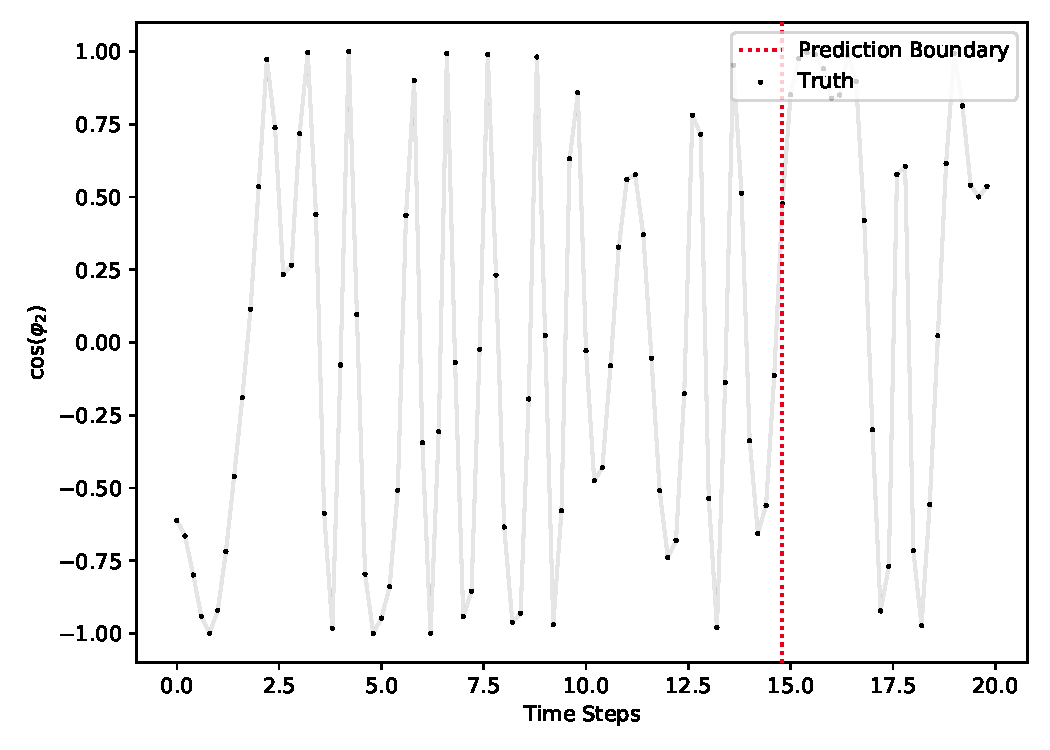
\includegraphics[width=\linewidth]{figures/experiments/environments/observations-acrobot-gym-N0-D2.pdf}
			\end{subfigure}%
			~
			\begin{subfigure}{0.5\linewidth}
				\centering
				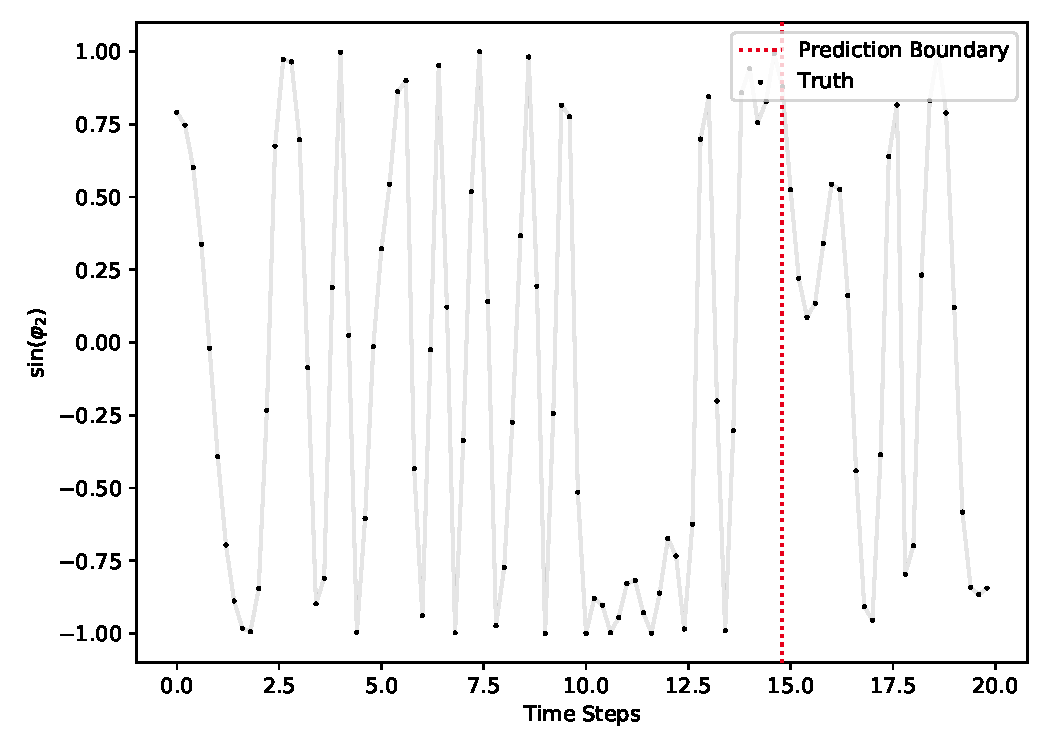
\includegraphics[width=\linewidth]{figures/experiments/environments/observations-acrobot-gym-N0-D3.pdf}
			\end{subfigure} \\
			\begin{subfigure}{0.5\linewidth}
				\centering
				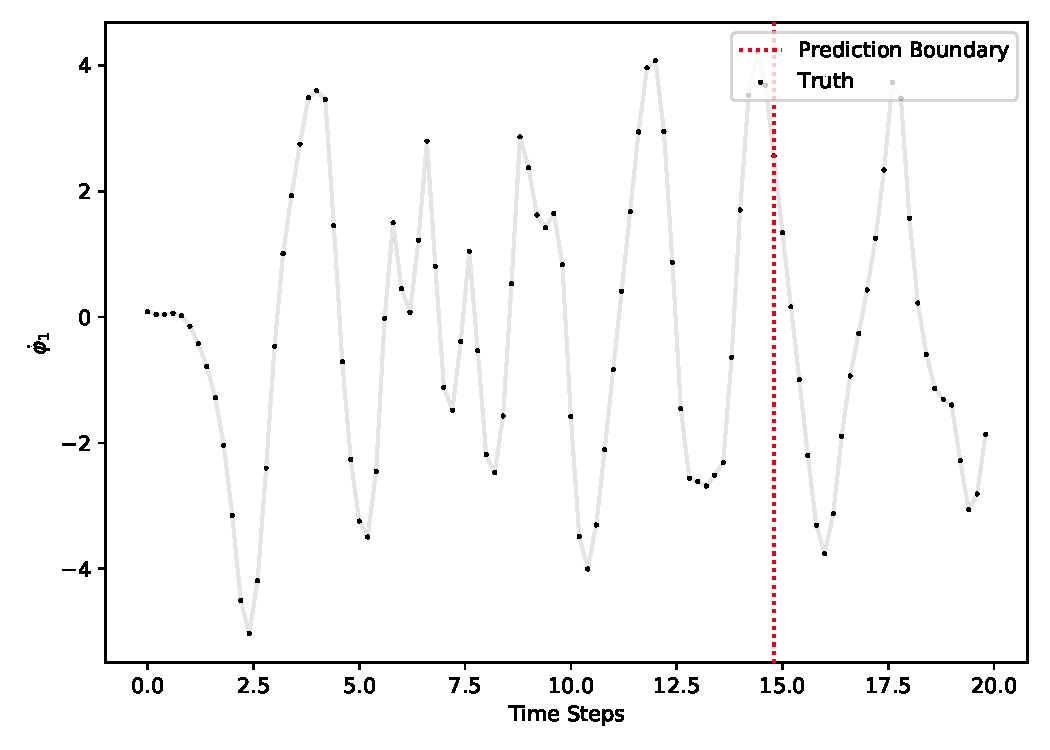
\includegraphics[width=\linewidth]{figures/experiments/environments/observations-acrobot-gym-N0-D4.pdf}
			\end{subfigure}%
			~
			\begin{subfigure}{0.5\linewidth}
				\centering
				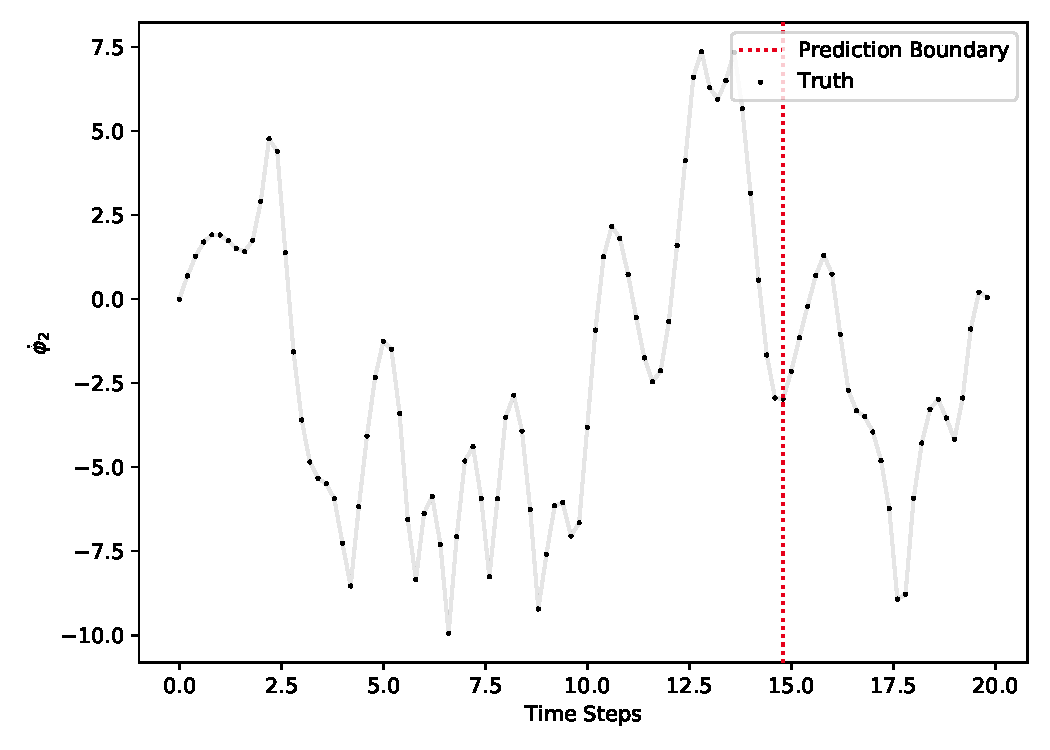
\includegraphics[width=\linewidth]{figures/experiments/environments/observations-acrobot-gym-N0-D5.pdf}
			\end{subfigure}
			\caption{Plot of the raw data used for training the Gym double pendulum environment. The black dots represent the actual data points, all before the red prediction boundary are used for training, the rest for validation. The faint gray line emphasizes the connection between the data points and that they are actually generated from a dynamical system.}
			\label{fig:envDoublePendulumGym}
		\end{figure}
	% end
% end

\section{Experiments with Hyperparameters}
	% Probably more if I can run more experiments… But all other hyperparameters are not as interesting.

	\todo{Exp: Hyper-experiments}

	\subsection{Influence of the Latent Dimensionality}
		\label{subsec:experimentLatentDim}

		\todo{Exp Hyper: Latent Dim}
	% end
% end
